 
\documentclass[english, nofootinbib]{revtex4-1}  % defines the basic parameters of the document
% if you want a single-column, remove reprint

% allows special characters (including æøå)
\usepackage[utf8]{inputenc}
%\usepackage [norsk]{babel} %if you write norwegian
\usepackage[english]{babel}  %if you write english


%% note that you may need to download some of these packages manually, it depends on your setup.
%% I recommend downloading TeXMaker, because it includes a large library of the most common packages.

\usepackage{physics,amssymb}  % mathematical symbols (physics imports amsmath)
\usepackage{graphicx}         % include graphics such as plots
\usepackage{xcolor}           % set colors
\usepackage{hyperref}         % automagic cross-referencing (this is GODLIKE)

\usepackage{tikz}             % draw figures manually
\usepackage{listings}         % display code
\usepackage{subfigure}        % imports a lot of cool and useful figure commands

\usepackage{amsmath,varioref,verbatim,amsfonts,geometry}

% defines the color of hyperref objects
% Blending two colors:  blue!80!black  =  80% blue and 20% black
\hypersetup{ % this is just my personal choice, feel free to change things
    colorlinks,
    linkcolor={red!50!black},
    citecolor={blue!50!black},
    urlcolor={blue!80!black}}

%% Defines the style of the programming listing
%% This is actually my personal template, go ahead and change stuff if you want
\lstset{ %
	inputpath=,
	backgroundcolor=\color{white!88!black},
	basicstyle={\ttfamily\scriptsize},
	commentstyle=\color{magenta},
	language=Python,
	morekeywords={True,False},
	tabsize=4,
	stringstyle=\color{green!55!black},
	frame=single,
	keywordstyle=\color{blue},
	showstringspaces=false,
	columns=fullflexible,
	keepspaces=true}

\def\bibsection{\section*{References}}

%% USEFUL LINKS:
%%
%%   UiO LaTeX guides:        https://www.mn.uio.no/ifi/tjenester/it/hjelp/latex/ 
%%   mathematics:             https://en.wikibooks.org/wiki/LaTeX/Mathematics

%%   PHYSICS !                https://mirror.hmc.edu/ctan/macros/latex/contrib/physics/physics.pdf

%%   the basics of Tikz:       https://en.wikibooks.org/wiki/LaTeX/PGF/TikZ
%%   all the colors!:          https://en.wikibooks.org/wiki/LaTeX/Colors
%%   how to draw tables:       https://en.wikibooks.org/wiki/LaTeX/Tables
%%   code listing styles:      https://en.wikibooks.org/wiki/LaTeX/Source_Code_Listings
%%   \includegraphics          https://en.wikibooks.org/wiki/LaTeX/Importing_Graphics
%%   learn more about figures  https://en.wikibooks.org/wiki/LaTeX/Floats,_Figures_and_Captions
%%   automagic bibliography:   https://en.wikibooks.org/wiki/LaTeX/Bibliography_Management  (this one is kinda difficult the first time)
%%   REVTeX Guide:             http://www.physics.csbsju.edu/370/papers/Journal_Style_Manuals/auguide4-1.pdf
%%
%%   (this document is of class "revtex4-1", the REVTeX Guide explains how the class works)


%% CREATING THE .pdf FILE USING LINUX IN THE TERMINAL
%% 
%% [terminal]$ pdflatex template.tex
%%
%% Run the command twice, always.
%% If you want to use \footnote, you need to run these commands (IN THIS SPECIFIC ORDER)
%% 
%% [terminal]$ pdflatex template.tex
%% [terminal]$ bibtex template
%% [terminal]$ pdflatex template.tex
%% [terminal]$ pdflatex template.tex
%%
%% Don't ask me why, I don't know.

\begin{document}



\title{Project 1}
\date{\today}               
\author{Ragnhild Wisted}
\affiliation{FYS3150, fall semester 2020} 
%\email{ragnhwis@student.matnat.uio.no}


\newpage

\begin{abstract}
We have developed two tridiagonal matrix algorithms for solving the one-dimensional general Poisson equation, one general and one specific. We then used these algorithms to study the correlation between the number of FLOPs required and the CPU time, and compared them to a LU decomposition method. The general algorithm required 1.5 times more FLOPs than the specific, and this was reflected in our results. For $n = 10^7$, the CPU times for the general solver was $1.28924\cdot 10^6$ microseconds, and for the specified solver it was $2.89226\cdot 10^5$ microseconds. While we expected the numerical precision to decrease as $n > 10^4$, this did not happen in our calculations. This is suspicious, and might indicate that something has gone wrong in our code.
\end{abstract}


\maketitle                                % creates the title, author, date & abstract
\section{Introduction}
The second derivative of a function $f(x)$ can be expressed as
\begin{equation} \label{eq: second derivative}
f''(x) = \lim_{h\rightarrow 0}\frac{f(x+h)-2f(x)+f(x-h)}{h^2},
\end{equation}
where $h$ is the step length between derivation points. Mathematically we would say that as $h$ becomes infinitely smaller, the approximation becomes more accurate. Nowadays however, these kinds of calculations are usually done on computers, and there is a limited amount of numbers that can be represented exactly in a computer. This leads to round-off errors, which will  accumulate when the number of integration points on a given interval increases, i.e. when the step length $h$ decreases. This means that paradoxically, as the theoretical mathematical precision increases, we see an increasing loss of numerical precision. In other words, just decreasing the step length $h$ will not necessarily lead to more accurate results.  

The goal of this project is explore how numerical errors can accumulate, while also becoming more familiar with concepts like pointers and memory allocation in C++, how the number of floating point operations (FLOPs) impact CPU time, and getting started with writing programs in C++. To achieve this, we will study the general one-dimensional Poisson equation,
\begin{equation} \label{eq: Poisson}
-\frac{d^2 u}{dx^2} = f(x).
\end{equation}

We will solve this for $x \in [0,1]$, with the boundary conditions $u(0)=u(1) = 0$. We assume that the source term is 
\begin{equation} \label{eq: f(x)}
f(x) = 100 e^{-10x}.
\end{equation}
This means that equation \ref{eq: Poisson} has a closed-form solution given by 
\begin{equation}\label{eq: u_analytic}
u(x) = 1-(1-e^{-10})x - e^{-10x}.
\end{equation}
We will write two algorithms for solving $u(x)$, one general and one for our specific case. To check if our algorithms work as intended we will plot the numerical solutions with the exact solution. The plots will be presented in section \ref{section: results}. 

We will then compare the maximum relative error of the numerical calculations from our two algorithms and study the correlation between the step length $h$ and the maximum value of the relative error.

Finally we will then study whether the number of floating point operations (FLOPs) required in two different algorithms impact the CPU time, and compare them to a LU decomposition method using the two functions \textbf{ludcmp()} and \textbf{lubksb()} from the external library \textbf{lib.cpp} found at the course's github repository.\cite{lib} 


\section{Method}


\subsection{Discretize the equation}
We define the discretized approximation to $u$ as $v_i$, and use equation \ref{eq: second derivative} to approximate the second derivative of $u$ with the following three point formula,
\begin{equation} \label{eq:u_discretized}
-v_i'' = -\frac{v_{i+1}+v_{i-1} - 2v_i}{h^2} = f_i \;\;\;\;\;\; \text{for $i = 1, \dots, n$},
\end{equation}
where $f_i = f(x_i)$. This discretized approximation has $n$ grid points $x_i = ih$ in the interval from $x_0 = 0$ to $x_{n+1} = 1$, with the step size being defined as $h = 1/n$. Our previous boundary conditions have now become $v_0 = v_{n+1} = 0$. 

We multiply equation \ref{eq:u_discretized} with $h^2$:
\begin{equation} \label{eq: u=h2f}
v_{i+1} + v_{i-1} - 2v_i = h^2 f_i.
\end{equation} 
We rename the above right side $g_i$:
\begin{equation} \label{eq: h2f=g}
h^2 f_i = g_i.
\end{equation}
Now we see that we end up with a set of equations
\begin{equation}
\begin{aligned}
i = 1 &\rightarrow v_2 -2v_1 + u_v = g_1\\
i = 2 &\rightarrow v_3 -2v_2 + v_1 = g_2\\
\vdots \\
i = n &\rightarrow v_{n+1} -2v_{n} + v_{n-1} = g_{n}
\end{aligned}
\end{equation}
We remember that $v_0 = v_{n+1} = 0$.

Now define a tridiagonal Töplitz matrix $\bf{A}$, which we see arises from the discretization of the second derivative:
$$
\bf{A} = \begin{bmatrix}
-2 & 1 & 0 & 0 & \cdots & 0\\
1 & -2 & 1 & 0 & \cdots & 0\\
0 & 1 & -2 & 1 & \cdots & 0\\
\vdots &\vdots & \vdots & \vdots & \cdots & \vdots \\
0 & \cdots & 0 & 1 & -2 & 1\\
0 & \cdots & 0 & 0 & 1 & -2
\end{bmatrix}
$$

Now we define two vectors
\begin{equation}
\bf{v}^T = [v_1, v_2, \dots , v_{n}]
\end{equation}
and
\begin{equation}
\bf{g}^T = [g_1, g_2, \dots , g_{n}]
\end{equation}
Now we see that equations \ref{eq: u=h2f} is equivalent to 
\begin{equation}
\bf{A}\bf{v} = \bf{g}.
\end{equation}

\subsection{The general algorithm}
Now we want to create an algorithm for solving this linear set of equations. We begin by looking at $\bf{A}$ for the case $n = 4$:
$$
\bf{A} = \begin{bmatrix}
d_1 & e_1 & 0 & 0\\
e_1 & d_2 & e_2 & 0\\
0 & e_2 & d_3 & e_3\\
0 & 0 & e_3 & d_4
\end{bmatrix}
$$
We see that all the information we need can be stored in two vectors $\bf{d}$ and $\bf{e}$:
\begin{equation}
\bf{d}^T = [d_1, d_2, \dots, d_{n}]
\end{equation}

\begin{equation}
\bf{e}^T = [e_1, e_2, \dots, e_{n-1}]
\end{equation}
Written out explicitly, $\bf{Av} = \bf{g}$ is then
\begin{equation}
\begin{aligned}
d_1\cdot v_1 + e_1\cdot v_2 + 0 + 0 &= g_1\\
e_1\cdot v_1 + d_2\cdot v_2 + e_2\cdot v_3 + 0 &= g_2\\
0 + e_2\cdot v_2 + d_3\cdot v_3 + e_3 \cdot v_4 &= g_3\\
0 + 0 + e_3\cdot v_3 + d_4 \cdot v_4 &= g_4
\end{aligned}
\end{equation}
If we leave out $\bf{v}$ this can be written as a matrix
$$
\begin{matrix}
d_1 & e_1 & 0 & 0 & g_1\\
e_1 & d_2 & e_2 & 0 & g_2\\
0 & e_2 & d_3 & e_3 & g_3\\
0 & 0 & e_3 & d_4 & g_4
\end{matrix}
$$

After Gaussian elimination this matrix has the form
$$
\begin{matrix}
d_1 & e_1 & 0 & 0 & g_1\\
0 & \tilde{d}_2 & e_2 & 0 & \tilde{g}_2\\
0 & 0 & \tilde{d}_3 & e_3 & \tilde{g}_3\\
0 & 0 & 0 & \tilde{d}_4 & \tilde{g}_4
\end{matrix}
$$
where the new vectors $\bf{\tilde{d}}$ and $\bf{\tilde{g}}$ are found by forward substitution:
\begin{equation} 
\begin{aligned}
\tilde{d}_i &= d_i - e_{i-1}^2/\tilde{d}_{i-1}\\
\tilde{g}_i &= g_i - e_{i-1}\cdot \tilde{g}_{i-1}/\tilde{d}_{i-1}
\end{aligned}
\end{equation}
with initial conditions $\tilde{d}_1 = d_1$ and $\tilde{g}_1 = g_1$.

The solution $u_i$ can then be found by using backwards substitution:
\begin{equation}
u_i = (\tilde{g}_i - e_i u_{i+1})/\tilde{d}_i.
\end{equation}

Our complete general algorithm (which is a version of the Thomas algorithm) is then
\begin{equation} 
\begin{aligned}
\tilde{d}_i &= d_i - e_{i-1}^2/\tilde{d}_{i-1}\\
\tilde{g}_i &= g_i - e_{i-1}\cdot \tilde{g}_{i-1}/\tilde{d}_{i-1}\\
v_i &= (\tilde{g}_i - e_i v_{i+1})/\tilde{d}_i
\end{aligned}
\end{equation}
These three steps require $3(n-2)$ (as the initial conditions $v_0 = v_{n+1} = 0$ are known) FLOPs each (one subtraction, one multiplication and one division). When $n$ is a high number, this is $\sim 3n$ per step, for a total of $\sim 9n$ FLOPs.\\

\subsection{The spesific algorithm}
In the case of our specific triangular matrix, we know that all entries $e_i = 1$. This means that $\tilde{d}_i$ is simply found by $\tilde{d}_i = d_i -1/\tilde{d}_{i-1}$. This has an analytical expression,
\begin{equation} \label{eq: d_i}
\tilde{d}_i = -\frac{(i+1)}{i}.
\end{equation}
$\bf{\tilde{g}}$ is then found by the now simplified forward substitution,
\begin{equation}
\tilde{g}_i = g_i - \tilde{g}_{i-1}/\tilde{d}_{i-1}
\end{equation}
with the initial condition $\tilde{g}_1 = g_1$.
The backwards substitution is then 
\begin{equation}
v_i = (\tilde{g}_i - v_{i+1})/\tilde{d}_i
\end{equation}
If $\bf{\tilde{d}}$ was pre-calculated, this would bring the number of FLOPs down to $4(n-2)\sim 4n$. However, in our program we ended up calculating $\tilde{d}_i$ in each iteration, and thus the total number of FLOPs is $\sim 6n$.
\subsection{Evaluating the relative error}
We have an analytical solution to our equation, which means that we can use the computed solution and the exact solution to evaluate the relative error $\epsilon$ in our solvers:
\begin{equation}
\epsilon = \abs{\frac{u_{\textrm{computed}}-u_{\textrm{exact}}}{u_{\textrm{exact}}}}
\end{equation}
We compute the logarithm of the relative error,
\begin{equation}
\epsilon_i = \log_{10}\left(\abs{\frac{v_i-u_i}{u_i}}\right),
\end{equation}
and study it as a function of $\log_{10}(h)$. Here, $v_i$ is the computed solution and $u_i$ is the exact, analytical solution. We choose to use the specific solver for this.
The results are presented in table \ref{table:relative_error}.


\subsection{Implementation}
In our program we defined  six vectors for the general solver, $\bf{g}$, $\bf{\tilde{g}}$, $\bf{d}$, $\bf{\tilde{d}}$, $\bf{e}$ and $\bf{u}$. The specific solver only needed four, namely $\bf{g}$, $\bf{\tilde{g}}$, $\bf{\tilde{d}}$, and $\bf{u}$. 
We created a function for the general and one for the specific algorithm. In order to compare the numerical results with the exact solution (equation \ref{eq: u_analytic}), we created a function to write the following variables to a data file: $n$, $\log_{10}(h)$, $x_i$, the exact solution $u(x_i)$, the general solution $v_{general}(x_i)$, its maximum relative error $\epsilon_{general}$, the specific solution $v_{specific}(x_i)$, its maximum relative error $\epsilon_{specific}$, the solution from the LU decomposition method $v_{LU}$, and its maximum relative error $\epsilon_{LU}$. This was done to be able to plot our results with matplotlib in python. 

The CPU time of each method was found by using the chrono function 
\begin{verbatim}
high_resolution_clock,
\end{verbatim}
and the time was found in microseconds (ms). In order to get a more accurate sense of the CPU time, we ran the calculations 10 times and used the median time. To find the median, we used a pre-made function to find the median of an unsorted array.\cite{median} To spending unnecessary time writing to file, we made sure that only the final run wrote the data to file.

\section{Results} \label{section: results}

The results of comparing our numerical solutions to the exact solution of $u(x)$ are shown in figures \ref{fig:n=10}, \ref{fig:n=100} and \ref{fig:n=1000}. 
The maximum relative error $\epsilon$ is presented as a function of $\log_{10}(h)$ in table \ref{table:relative_error}. The different CPU times are shown in table \ref{table:CPU_time}.

\begin{table}[h!]
\centering
\setlength{\tabcolsep}{12pt}
 \begin{tabular}{l  l  l} 
 \hline
n & $\log_{10}(h)$ & Maximum $\epsilon$ \\ [0.5ex] 
 \hline\hline
$10$ & -1.0 & 0.327572\\ 

$10^2$& -2.0 & 0.037856\\

$10^3$ & -3.0 & 0.003853 \\
 
$10^4$& -4.0 & 0.000386 \\

$10^5$ & -5.0 & 3.9e-05 \\ 

$10^6$ & -6.0 & 4e-06 \\ 

$10^7$ & -7.0 & 1e-06 \\ 
\hline
\hline
\end{tabular}
\caption{Maximum value of the relative error $\epsilon$ as a function of the step size $h$. The general algorithm was used to extract the values.}
\label{table:relative_error}
\end{table}


\begin{table}[h!]
\centering
\setlength{\tabcolsep}{12pt}
 \begin{tabular}{l  l  l  l} 
 \hline
n & CPU time LU decomposition [ms] & CPU time general solver [ms] & CPU time specified solver [ms]\\ [0.5ex] 
 \hline\hline
$10$ & 0 & 0 & 0\\ 

$10^2$& $1.985\cdot 10^3$ & 0 & 0  \\

$10^3$ & $2.91087\cdot 10^6$ & 0 & 0  \\ 

$10^4$ & - & $4.965\cdot 10^2$ & 0 \\ 

$10^5$ & - & $6.483 \cdot 10^3$ & $2.9895\cdot 10^3$ \\ 

$10^6$ &- & $5.44835\cdot 10^4$ & $2.8424\cdot 10^4$ \\ 

$10^7$ &- & $1.28924\cdot 10^6$ & $2.89226\cdot 10^5$ \\ 
\hline
\hline
\end{tabular}
\caption{CPU time for the different solvers, given in microseconds.}
\label{table:CPU_time}
\end{table}

\newpage
\begin{figure}[h!]
        \centering 
        %Scale angir størrelsen på bildet. Bildefilen må ligge i samme mappe som tex-filen. 
        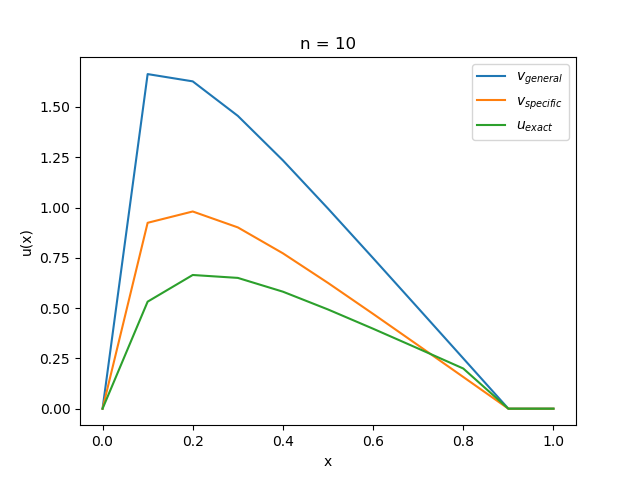
\includegraphics[scale=0.8]{FYS3150_oblig1_1.png} 
        \caption{Comparison of the numerical and exact solution with $n = 10$.}
        %Label gjør det enkelt å referere til ulike bilder.
        \label{fig:n=10}
\end{figure}

\begin{figure}[h!]
        \centering 
        %Scale angir størrelsen på bildet. Bildefilen må ligge i samme mappe som tex-filen. 
        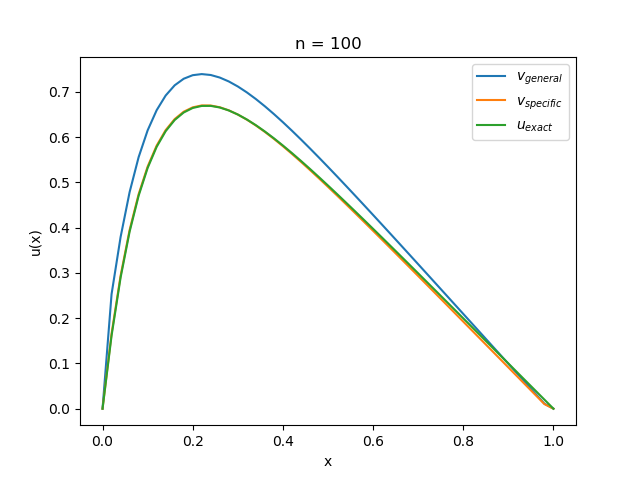
\includegraphics[scale=0.8]{FYS3150_oblig1_2.png} 
        \caption{Comparison of the numerical and exact solution with $n = 10^2$.}
        %Label gjør det enkelt å referere til ulike bilder.
        \label{fig:n=100}
\end{figure}

\begin{figure}[h!]
        \centering 
        %Scale angir størrelsen på bildet. Bildefilen må ligge i samme mappe som tex-filen. 
        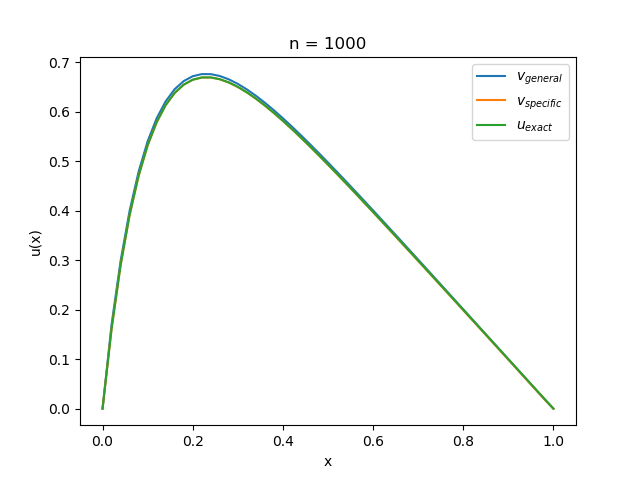
\includegraphics[scale=0.8]{FYS3150_oblig1_3.png} 
        \caption{Comparison of the numerical and exact solution with $n = 10^3$.}
        %Label gjør det enkelt å referere til ulike bilder.
        \label{fig:n=1000}
\end{figure}


\begin{figure}[h!]
        \centering 
        %Scale angir størrelsen på bildet. Bildefilen må ligge i samme mappe som tex-filen. 
        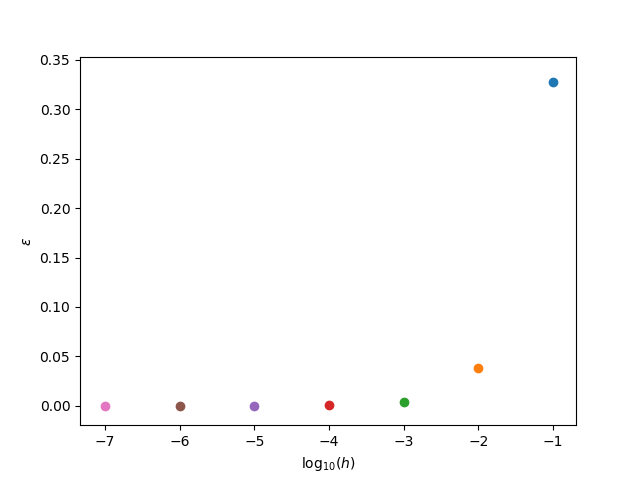
\includegraphics[scale=0.8]{error_plot.png} 
        \caption{Logarithmic plot of the maximum relative error $epsilon$ as a function of $h$.}
        %Label gjør det enkelt å referere til ulike bilder.
        \label{fig:error_plot}
\end{figure}




\newpage
\section{Discussion/Conclusion}
From the plots of the numerical and analytical solutions of the equation, we can see that both our algorithms are good approximations, especially for $n \geq 1000$. In figure \ref{fig:n=10} something happens that makes all the functions go to 0 one step too early, this could be a mistake in the method for extracting the data. 


The relative error $\epsilon$ as function of step size $h$ in figure \ref{fig:error_plot} is unexpected. What we expect is that the relative error has its minimum around $\log_{10}(h) = -4$, and increases for smaller step lengths due to accumulation of numerical imprecision. In our plot the relative error appears to stay small for increasingly smaller values of $h$. This is a bit worrying, and might indicate that something is wrong in our code. From table \ref{table:relative_error} we see that $\epsilon$ behaves as expected until $n = 10^4$, but for the higher values of $n$ they seem too small. 

As for the CPU time, we see that the LU decomposition method, which requires an entire $n\cross n$ matrix, is substantially slower than our solvers. In our code, the LU decomposition method was not viable for $n \geq 10^4$. We also see that of our methods, the specific solver (which requires less FLOPs) is faster than the general solver.

\begin{thebibliography}{}

\bibitem[course library (2020)]{lib} Course git repository: \url{https://github.com/CompPhysics/ComputationalPhysics/tree/master/doc/Programs/LecturePrograms/programs/LinAlgebra/cpp}

\bibitem[median function (2020)]{median} Median function: \url{https://xoax.net/cpp/ref/cpp_examples/incl/mean_med_mod_array/}

\end{thebibliography}


\end{document}




































